\section{Experiments}
\label{sec:experiments}

\subsection{Setup}

Section~\ref{sec:dataset} describes the data, protocol and metrics.
Section~\ref{sec:method} describes the model, optimizer, batch size
and augmentation. We found no canonical chip-ID overlap between the
official test subset and the reconstructed weak or hand training and
validation roles. The georeferenced checks likewise found no positive-area
interior intersections above the specified tolerance ($10^{-8}$ degrees
on both axes) across 425,250 generalist test-to-role tile pairs. Boundary
contacts or sub-tolerance intersections occur for 73 test chips against
weak training and 35 against hand training. These checks describe the
recorded membership and current raster grids. Shared scene context,
adjacency and preprocessing exposure remain sources of dependence.

\subsection{LOCO Results}
\label{sec:loco}

Table~\ref{tab:a1test} reports the nine recoverable event--seed comparisons
out of 30 planned, spanning seven events and 51 of the 90 unique
official test chips. The fixed generalist reaches pooled IoU 0.676564
and F1 0.807084 over all 90 chips. Two official chips contain no valid
pixels and contribute zero counts. Ghana, India and Paraguay have no
recoverable LOCO results under the frozen selection.

\begin{table}[!htbp]
\caption{Pooled water-class IoU on each event's official test chips.
Dashes indicate unavailable event-excluded results. Differences use
full-precision scores.}
\label{tab:a1test}
\centering\small
\begin{tabular}{@{}lrrrrr@{}}
\toprule
Event & Test chips & Seed & Generalist & LOCO & $\Delta$ \\
\midrule
Ghana & 11 & -- & 0.5793 & -- & -- \\
India & 14 & -- & 0.6655 & -- & -- \\
Mekong & 6 & 43 & 0.8443 & 0.8487 & $+0.0044$ \\
Mekong & 6 & 44 & 0.8443 & 0.8377 & $-0.0066$ \\
Nigeria & 4 & 43 & 0.8831 & 0.8912 & $+0.0080$ \\
Pakistan & 6 & 43 & 0.2690 & 0.2354 & $-0.0336$ \\
Pakistan & 6 & 44 & 0.2690 & 0.2943 & $+0.0253$ \\
Paraguay & 14 & -- & 0.6641 & -- & -- \\
Somalia & 6 & 42 & 0.5027 & 0.5151 & $+0.0124$ \\
Spain & 6 & 42 & 0.7237 & 0.7215 & $-0.0022$ \\
Sri Lanka & 9 & 42 & 0.8353 & 0.8377 & $+0.0024$ \\
USA & 14 & 42 & 0.5525 & 0.5522 & $-0.0003$ \\
\bottomrule
\end{tabular}

\end{table}

For USA seed 42, the historical evaluator used an interrupted run's
\texttt{best.ckpt}. The reconstruction uses the completed retry's
\texttt{best-v1.ckpt}, selected by its validation maximum. The two USA
scores consequently refer to different checkpoints. No all-event mean,
event ranking or three-seed interval is estimated from the surviving
runs.

\subsection{Interpolation vs. Generalization on Paired Test Chips}
\label{sec:sensitivity}

On the same test chips, five of the nine differences in Eq.~\ref{eq:paired} are positive
and four are negative, from $-0.033583$ to $+0.025312$.
Mekong and Pakistan each change sign between seeds 43 and 44.
Variation across generalist training runs remains unmeasured.

We recompute the difference after dropping each test chip in turn
from both models, leaving the weights, valid masks and threshold fixed.
Across 63 such omissions, seven of nine comparisons can reverse sign.
In Pakistan seed 44, one chip contains 171,908 of 198,897 labeled water
pixels. Removing that chip changes the difference from $+0.0253$ to
$-0.2220$. Figure~\ref{fig:chip-sensitivity} shows the full-chip
difference and the observed minimum and maximum under each single-chip
omission. These are deterministic sensitivity ranges on the observed
sample. They have no confidence-interval interpretation.

\begin{figure}[!htbp]
\centering
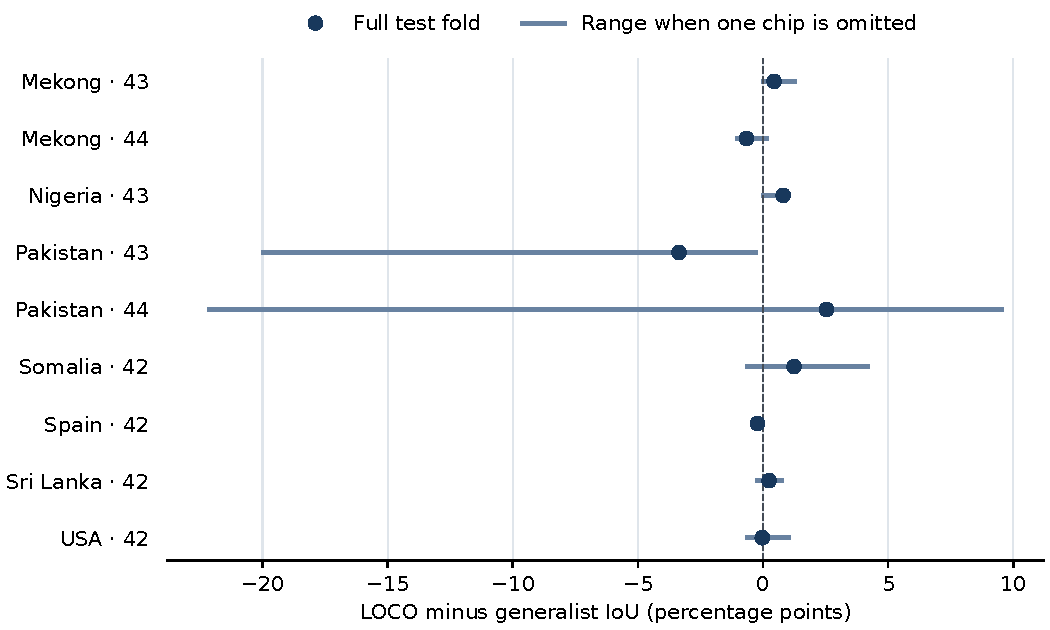
\includegraphics[width=\linewidth]{figures/chip_sensitivity.pdf}
\caption{Full-test paired water-IoU differences (dots) and the observed
minimum and maximum after omitting one test chip from both models
(horizontal ranges). The dashed line marks zero.}
\label{fig:chip-sensitivity}
\end{figure}

\subsection{Ablations}
\label{sec:ablations}

\paragraph{Two-stage training.}
We compare the two-stage scheme with a single-stage baseline trained
on hand labels only (Table~\ref{tab:two-stage}). These two seed-42
DeepLabV3+/ResNet-50 runs reached test IoUs of 0.6732 and 0.6766.
The fine-tuning settings recorded for the two runs were closely
matched, with different source snapshots. Weak labels provide a
greater variety of scenes than manual chips alone, a motivation for
pretraining. The numerical difference describes these two fits.

\begin{table}[!htbp]
\caption{Two-stage and hand-only DeepLabV3+/ResNet-50 runs, seed 42,
evaluated on the standard hand test split.}
\label{tab:two-stage}
\centering\small
\begin{tabular}{@{}lrr@{}}
\toprule
Training & IoU & F1 \\
\midrule
Single-stage (hand labels only) & 0.6732 & 0.8047 \\
Two-stage (weak $\to$ hand) & 0.6766 & 0.8071 \\
Difference & +0.0034 & +0.0024 \\
\bottomrule
\end{tabular}

\end{table}

\paragraph{Loss function.}
Table~\ref{tab:loss} gives the full sweep over 11 variants. The three
overlap-based losses (Focal-Tversky, Tversky and Dice) are within 0.001
validation IoU of each other. In this sweep their advantage over the
best BCE setting is about 0.04 IoU. Dice needs no imbalance
hyperparameter, which motivated its use in the event-held-out recipe.
BCE at weight 8.4, taken from the full-catalog label ratio, scored below
weight 4. The class-ratio heuristic was therefore a poor guide to the
best weight in this setting.

\begin{table}[!htbp]
\caption{Loss sweep on the 89-chip validation split using
DeepLabV3+/ResNet-34, seed 42, one run per variant on a Colab T4,
with a 40-epoch limit and early stopping (patience 8).}
\label{tab:loss}
\centering\small
\begin{tabular}{@{}lrr@{}}
\toprule
Loss & Val. IoU & Val. F1 \\
\midrule
Focal-Tversky ($\gamma=1.33$) & 0.6434 & 0.7830 \\
Tversky ($\alpha=0.3$, $\beta=0.7$) & 0.6427 & 0.7825 \\
Dice & 0.6425 & 0.7824 \\
Dice + Focal & 0.6261 & 0.7701 \\
Dice + BCE (weight 8.4) & 0.6066 & 0.7551 \\
BCE, positive weight 4 & 0.5988 & 0.7491 \\
BCE, positive weight 8.4 & 0.5525 & 0.7118 \\
Focal ($\alpha=0.25$) & 0.5428 & 0.7037 \\
Lov\'asz & 0.5136 & 0.6787 \\
BCE, positive weight 13 & 0.5107 & 0.6761 \\
BCE, positive weight 1 & 0.4749 & 0.6440 \\
\bottomrule
\end{tabular}

\end{table}
